\documentclass{standalone}

\usepackage{amssymb}
\usepackage{amsthm}
\usepackage{amsmath}


\usepackage{tikz}
\usetikzlibrary{shapes,backgrounds,calc,patterns}


\begin{document}
	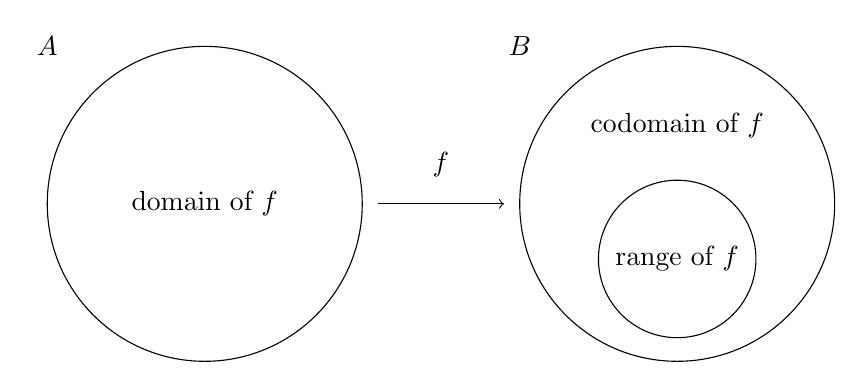
\begin{tikzpicture}
		\draw (-3,0) circle (2);
		\node at (-3,0) {domain of \(f\)};
		\node at (-5,2) {\(A\)};
		
		\draw (3,0) circle (2);
		\node at (3,1) {codomain of \(f\)};
		\node at (1,2) {\(B\)};	
		
		\draw (3,-.7) circle (1);
		\node at (3,-.7) {range of \(f\)};

		
		\draw[->] (-.8,0) -- (.8,0);
		\node at (0,.5) {\(f\)};	
	\end{tikzpicture}
	
	
	
\end{document}